\documentclass[12pt,letterpaper,noanswers]{exam}
\usepackage[usenames,dvipsnames,svgnames,table]{xcolor}
\usepackage[margin=0.9in]{geometry}
\renewcommand{\familydefault}{\sfdefault}
\usepackage{multicol}
\pagestyle{head}
\header{AM 111 Class 21}{}{Initial value problems: differential equations, p.\thepage}
\runningheadrule
\headrule
\usepackage{siunitx}
\usepackage{graphicx} % more modern
\usepackage{amsmath} 
\usepackage{amssymb} 
\usepackage{hyperref}
\usepackage{tcolorbox}
\usepackage{enumitem}
\def\mbf{\mathbf}
\newcommand{\vc}[1]{\boldsymbol{#1}}
\def\dsst{\displaystyle}
\DeclareMathOperator*{\argmin}{arg\,min} % thin space, limits underneath in displays
\usepackage{listings}

\begin{document}
 \pdfpageheight 11in 
  \pdfpagewidth 8.5in

\noindent 

\section*{Preliminaries}

\begin{itemize}
\itemsep0pt
\item Your project log is due Friday.
\item There is a skill check in the next class.
\end{itemize}


\noindent\textbf{Big picture}

Today: Sometimes explicit methods require very small step sizes to meet desired error tolerances.  What other options are there?

\vspace{0.2cm}
\hrule
\vspace{0.2cm}

\noindent \textbf{Skill check practice}

Given a differential equation for $(x(t),y(t))$ and an initial condition setting $(x_0,y_0)$, set up a pair of implicit equations for $x_1, y_1$ using the backwards Euler method.

\[\displaystyle\begin{array}{l} dx/dt = 3x - 2xy \\
dy/dt= 2y - xy - y^2 \end{array}\]

with $x(0) = 3, y(0) = 2$.

\vspace{0.2cm}
\hrule
\vspace{0.2cm}

\noindent \textbf{Skill check solution}

$x_1 = x_0 + h (3x_1 - 2x_1 y_1)$


$y_1 = y_0 + h (2y_1 - x_1 y_1 - y_1^2)$

Substituting the information we were given,

$x_1 = 3 + h (3x_1 - 2x_1 y_1)$


$y_1 = 2 + h (2y_1 - x_1 y_1 - y_1^2)$




\vspace{0.2cm}
\hrule
\vspace{0.2cm}


\section*{Ordinary differential equations}

\subsection*{Systems of first order equations}
% \begin{tcolorbox}
% The two methods we have encountered so far work for initial value problems, which involve first order differential equations.

% A second order differential equation can be turned into a \textbf{system} of two first order differential equations (and an $n$th order differential equation into  a system of $n$ first order equations).
% \end{tcolorbox}
\begin{enumerate}[resume]
\item Convert the second-order differential equation $y'' = a(y')^2 +yy' - \cos t$ to a system of two first order equations.
\begin{parts}
\item Set $y_1 = y$ and define the new variable $y_2 = y'$.  Rewrite the equation above, by replacing $y''$ with $y_2'$.  Replace $y'$ with $y_2$.  Replace $y$ with $y_1$.
\vspace{1cm}
\item Write down your system.  $y_1' = y_2$ is the first equation in the system.  $y_2' = ??$ is the second equation.
\vspace{1.5cm}
\end{parts}
\item Apply one step of Euler's method to initial value problem \[\left\{\begin{array}{l}
y_1' = y_2 - y_1^2 \\
y_2' = y_1 -ty_2^3 \\
y_1(1) = 0 \\
y_2(1) = 3 \end{array}\right.\]
$\begin{array}{l}
w_{0,1} = 0\\
w_{0,2} = 3
\end{array}$. Set up expressions for $\begin{array}{l}
w_{1,1}\\
w_{1,2}
\end{array}$
\vspace{1in}
\end{enumerate}




% \begin{tcolorbox}
% Explicit \textbf{Runge-Kutta} methods use intermediate estimates of $y$ in the interval $[t_k,t_{k+1}]$ in order to create $\psi(t_k,w_k,h)$.  
% \begin{itemize}
% \itemsep0pt
%     \item Explicit trapezoid is a Runge-Kutta method.  So is the midpoint method.  Recall that their global truncation error is 2nd order, so it is called second order Runge-Kutta methods.
%     \item The \textbf{classical fourth-order Runge-Kutta method} (RK4) is given by 
    
%     $s_1 = f(t_k,w_k)$, 
    
%     $s_2 = f(t_k+h/2,w_k+\frac{h}{2}s_1)$
    
%     $s_3 = f(t_k + h/2,w_k + \frac{h}{2}s_2)$
    
%     $s_4 = f(t_k+h, h_k + hs_3)$
    
%     $\psi(t_k,w_k,h) = \frac{1}{6}(s_1+2s_2+2s_3+s_4)$
% \end{itemize}

% We will not Taylor expand to show this has local truncation error of 5th order.
% \end{tcolorbox}
\begin{enumerate}[resume]
\item Let $\frac{dy}{dt} = ty$, $y(0) = 1$.  The Python code below implement forward Euler to estimate $y(1)$ using steps of size $0.1$.

\begin{lstlisting}
import numpy as np

def forward_euler(x,f,t,h):
    return x + h*f(t,x)

def odef(t,x):
    # define the differential equation: dx/dt = t*x
    return t*x

x0 = 1
tspan = 1
h = 0.1
# number of timesteps:
nt = int(np.floor(tspan/h))
t = np.arange(nt)*h
x = np.zeros([nt,1])
x[0,:] = x0
for n in np.arange(nt-1):
    x[n+1] = forward_euler(x[n],odef,t[n],h)
    
\end{lstlisting}

Modify the code to use RK4.


\vspace{1in}

\item How would the code need to change to solve a system, $\frac{dy_1}{dt} = t(y_1+y_2)$, $\frac{dy_2}{dt} = \sin y_2$, $y_1(0) = 1, y_2(0) = 1$?
\end{enumerate}

\subsection*{Variable step size methods}

% Main idea: approximate the error on the current step, $e_k$.  If $e_k$ (absolute) and/or $e_k/\vert w_k\vert$ (relative) error is below tolerance, keep the step.  Otherwise, lower the step size.  If error is far below tolerance, increase the step size for the next step.

% Goal: use large step sizes while meeting error tolerances.

% How is the error estimated?

% In our integration methods, we used the same method with two different step sizes to approximate error.  For this problem, we use methods with two different orders: and RK 23 pair, or an RK 45 pair.

\begin{enumerate}[resume]
\item Combine explicit trapezoid (order 2) with a rule similar to Simpson's (order 3).

Let

$s_1 = f(t_k,w_k)$

$s_2 = f(t_k + h, w_k + hs_1)$

$s_3 = f\left(t_k+ h/2, w_k + h/2\frac{s_1+s_2}{2}\right)$

$w_{k+1} = w_k + h\frac{s_1+s_2}{2}$

$z_{k+1} = w_k + h\frac{s_1+4s_3+s_2}{6}$.

\begin{enumerate}
\item How many additional function evaluations (evaluations of $f$) were used to create $w_{k+1}, z_{k+1}$ compared to just creating $w_{k+1}$?
\vspace{1cm}

\item How can you use $w_{k+1}$ and $z_{k+1}$ to approximate the error?
\vspace{1cm}

\item Does it make more sense to use $w_{k+1}$ or $z_{k+1}$ as the starting value for the next step?
\vspace{1cm}
\end{enumerate}
\item Matlab's \texttt{ode23} (Bogacki-Shampine order 2/order 3 embedded pair)

$s_1 = f(t_k,w_k)$

$s_2 = f(t_k + \frac{h}{2}, w_k + \frac{h}{2}s_1)$

$s_3 = f(t_k + \frac{3h}{4}, w_k + \frac{3h}{4}s_2)$

$z_{k+1} = w_k + h\frac{2s_1+3s_2+4s_3}{9}$.

$s_4 = f(t_k+ h, z_{k+1})$

$w_{k+1} = w_k + h\frac{7s_1+6s_2+8s_3+3s_4}{24}$

$z_{k+1}$ is order 3 and $w_{k+1}$ is order 2.

Compare $s_1$ and $s_4$.  This method design is called `first same as last' (FSAL).  What is that referring to?

\end{enumerate}

\subsection*{Stiff equations (Greenbaum and Chartier \S 11.4)}


\begin{enumerate}[resume]
\item For the system
\begin{align*}
    y_1' &= -100 y_1 + y_2 \\
    y_2' &= -0.1 y_2
\end{align*}
the exact solution is given by $y_2(t) = y_2(0)e^{-0.1t}$ and $y_1(t) = e^{-100t}(y_1(0) - 10y_2(0)/999)+e^{-0.1t}10y_2(0)/999$.
\begin{parts}
\item Let $y_1(0) = y_2(0) = 1$.  Based on the exact solution, how should $y_1$ and $y_2$ evolve with time?  Will their values increase or decrease?
\vspace{1cm}
\item In the plot below, using Euler's method with $h = 0.03$, how do the approximated solutions evolve with time?
\vspace{1cm}
\end{parts}
\end{enumerate}
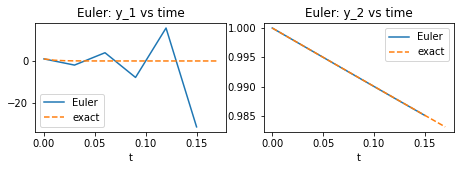
\includegraphics{img/C19stiff.png}
% \begin{tcolorbox}
% When equations have components evolving on very different time scales they are called \textbf{stiff} equations.
% \begin{itemize}
% \itemsep0pt
%     \item For the example of stiff equations above, Euler's method fails for step sizes above $h<0.02$: it fails by generating growth and oscillation instead of exponential decay.
%     \item Failure where the method does not match the actual long term behavior of the system is called \textbf{instability}.
% \end{itemize}
% \end{tcolorbox}
% \begin{tcolorbox}
% To assess stability of the method, use the test equation $dy/dt = \lambda y$, with $\lambda \in \mathbb{C}$.
% \begin{itemize}
% \itemsep0pt
% \item For $\lambda = a + ib$ with $a,b\in\mathbb{R}$, the exact solution to the test equation is $y(t) = y_0e^{\lambda t} = y_0e^{at}e^{ibt} = y_0e^{at}(\cos bt + i \sin bt)$.  It decays to $0$ for $a<0$, which corresponds to the left half of the complex plane.
%     \item Apply a numerical method, with step size $h$, to the test equation.  Find the set of $h\lambda \in \mathbb{C}$ such that $y_k\rightarrow 0$ as $k\rightarrow\infty$.
%     \item This is the region of \textbf{absolute stability} of the method.
%     \item A method is called \textbf{A-stable} when the entire left half plane is in its region of absolute stability.
% \end{itemize}
% \end{tcolorbox}
\begin{enumerate}[resume]
    \item You applied the forward Euler method to $dy/dt = cy$ in a prior class.  For this method, with $dy/dt = \lambda y$, $y_{k+1} = y_0(1+h\lambda)^{k+1}$.  
    \begin{parts}
    \item Find a mathematical expression for the region of absolute stability (the set of $h\lambda \in \mathbb{C}$ such that $y_k\rightarrow 0$ as $k\rightarrow \infty$).
    \vspace{1in}
\item To help you plot this region in the complex plane, write $h\lambda = x + iy$, and find the set of points $(x,y)$ that satisfy the condition, then plot the region.
\vspace{2in}
    \end{parts}
\end{enumerate}




\subsection*{Implicit methods}
% \begin{tcolorbox}
% \begin{itemize}
% \itemsep0pt
%     \item Implicit methods are a class of methods that tend to have better stability properties than explicit methods.
%     \item The \textbf{backward Euler} method is $y_{k+1} = y_k + hf(t_{k+1},y_{k+1})$.  This is an \textbf{implicit} equation for $y_{k+1}$: $y_{k+1}$ is an unknown and appears on both sides of the equation.
%     \item Implicit Runge-Kutta (IRK) methods also exist (and the weights are related to Gaussian quadrature, see Greenbaum and Chartier \S 11.4.3).
% \end{itemize}
% \end{tcolorbox}

\begin{enumerate}[resume]
\item Let $\dfrac{dx}{dt} = -x^3/3 + x + \alpha$.  Set $\alpha = 2/3, x(0) = 2$.  
\begin{parts}
    \item Set up an implicit equation for finding $x_1$ using the backwards Euler method ($x_0 = x(0) = 2$).
    \vspace{1in}
    \item Identify a method could you use to solve for $x_1$.
    \vspace{1cm}
\end{parts}

\item (Greenbaum and Chartier \S 11.6 Q 16) A simple model for a muscle controlling a heart valve is given by \[\displaystyle\begin{array}{l} dx/dt = -x^3/3 + x + \alpha \\
d\alpha/dt= -\epsilon x \end{array}\]
where $x$ is the position of the muscle and $\alpha$ is the concentration of a chemical stimulus.

Let $\epsilon = 0.01, x(0) = 2, \alpha(0) = 2/3$.  Set up a pair of implicit equations for $x_1, \alpha_1$ using the backwards Euler method.  

Note: $x_{k+1} = x_k + hf(t_{k+1},x_{k+1},\alpha_{k+1})$, $\alpha_{k+1} = \alpha_k + hf(t_{k+1},x_{k+1},\alpha_{k+1})$ 
\vspace{1in}
\end{enumerate}
% \begin{tcolorbox}
% \begin{itemize}\itemsep0pt
%         \item To use backward Euler requires solving a nonlinear equation with one unknown at each step.  That means it requires the use of a root finding method.
%     \item When using an implicit method, it is typical to use an explicit method to make a guess of the value of $y_{k+1}$ (a \textbf{predictor step}), and then take a \textbf{corrector step} using the implicit method.
% \end{itemize}
% \end{tcolorbox}

\begin{enumerate}[resume]
    \item Apply the backwards Euler method to the test equation, $\frac{dy}{dt} = \lambda y$.
    \begin{parts}
    \item First find an expression for $y_{k+1}$ in terms of $y_k$.  Then find an expression for $y_{k+1}$ in terms of $h,\lambda,k, y_0$.
    \vspace{1in}
    \item Find a mathematical expression for the region of absolute stability.
    \vspace{1.5cm}
    \item To help you think about this region in the complex plane, again write $h\lambda = x + iy$.  Argue that for $x<0$ the condition you found will always be true.
    \vspace{1in}
    \end{parts}
    The backwards Euler method is A-stable.
\end{enumerate}

%\subsection*{Implementation considerations (Greenbaum and Chartier \S 11.2.8)}
\end{document}